	%% `template.tex', a bare-bones example employing the AIAA class.
%
% For a more advanced example that makes use of several third-party
% LaTeX packages, see `advanced_example.tex', but please read the
% Known Problems section of the users manual first.
%
% Typical processing for PostScript (PS) output:
%
%  latex template
%  latex template   (repeat as needed to resolve references)
%
%  xdvi template    (onscreen draft display)
%  dvips template   (postscript)
%  gv template.ps   (onscreen display)
%  lpr template.ps  (hardcopy)
%
% With the above, only Encapsulated PostScript (EPS) images can be used.
%
% Typical processing for Portable Document Format (PDF) output:
%
%  pdflatex template
%  pdflatex template      (repeat as needed to resolve references)
%
%  acroread template.pdf  (onscreen display)
%
% If you have EPS figures, you will need to use the epstopdf script
% to convert them to PDF because PDF is a limmited subset of EPS.
% pdflatex accepts a variety of other image formats such as JPG, TIF,
% PNG, and so forth -- check the documentation for your version.
%
% If you do *not* specify suffixes when using the graphicx package's
% \includegraphics command, latex and pdflatex will automatically select
% the appropriate figure format from those available.  This allows you
% to produce PS and PDF output from the same LaTeX source file.
%
% To generate a large format (e.g., 11"x17") PostScript copy for editing
% purposes, use
%
%  dvips -x 1467 -O -0.65in,0.85in -t tabloid template
%
% For further details and support, read the Users Manual, aiaa.pdf.


% Try to reduce the number of latex support calls from people who
% don't read the included documentation.
%

\typeout{}\typeout{If latex fails to find aiaa-tc, read the README file!}
%
\documentclass[]{aiaa-tc}% insert '[draft]' option to show overfull boxes

\usepackage[acronyms]{glossaries}
\usepackage{amsmath}
\usepackage{pgfplotstable}
\usepackage{array}
\usepackage[sort, numbers]{natbib}
\usepackage{pgfplotstable,filecontents}
\usepackage{csvsimple}
\usepackage{booktabs}
\usepackage{tikz}
\usetikzlibrary{shapes, arrows, positioning, decorations.markings, fit}
\makeglossaries

\tikzstyle{block} = [draw, rectangle, 
    minimum height=3em, minimum width=6em]
\tikzstyle{sum} = [draw, circle]
\tikzstyle{input} = [coordinate]
\tikzstyle{output} = [coordinate]
\tikzstyle{pinstyle} = [pin edge={to-,thin,black}]
\tikzstyle{vecArrow} = [thick, decoration={markings,mark=at position
   1 with {\arrow[semithick]{open triangle 60}}},
   double distance=1.4pt, shorten >= 5.5pt,
   preaction = {decorate},
   postaction = {draw,line width=1.4pt, white,shorten >= 4.5pt}]
\tikzstyle{innerWhite} = [semithick, white,line width=1.4pt, shorten >= 4.5pt]

\makeatletter
\csvset{
  autotabularcenter/.style={
    file=#1,
    after head=\csv@pretable\begin{tabular}{|*{\csv@columncount}{c|}}\csv@tablehead,
    table head=\hline\csvlinetotablerow\\\hline,
    late after line=\\,
    table foot=\\\hline,
    late after last line=\csv@tablefoot\end{tabular}\csv@posttable,
    command=\csvlinetotablerow},
  autobooktabularcenter/.style={
    file=#1,
    after head=\csv@pretable\begin{tabular}{*{\csv@columncount}{c}}\csv@tablehead,
    table head=\toprule\csvlinetotablerow\\\midrule,
    late after line=\\,
    table foot=\\\bottomrule,
    late after last line=\csv@tablefoot\end{tabular}\csv@posttable,
    command=\csvlinetotablerow},
}
\makeatother
\newcommand{\csvautotabularcenter}[2][]{\csvloop{autotabularcenter={#2},#1}}
\newcommand{\csvautobooktabularcenter}[2][]{\csvloop{autobooktabularcenter={#2},#1}}
\newcommand{\norm}[1]{\left\lVert#1\right\rVert}

\newacronym{bsfc}{BSFC}{brake specific fuel consumption}
\newacronym{ceg}{CEG}{Convex Engineering Group}
\newacronym{gp}{GP}{Geometric Program}
\newacronym{mc}{MC}{Monte Carlo}
\newacronym{sp}{SP}{Signomial Program}
\newacronym{rgp}{RGP}{Robust Geometric Program}
\newacronym{rsp}{RSP}{Robust Signomial Program}
\newacronym{ro}{RO}{Robust Optimization}
\newacronym{so}{SO}{Stochastic Optimization}
\newacronym{mdo}{MDO}{Multidisciplinary Design Optimization}
\newacronym{dc}{DC}{difference-of-convex}
\newacronym{nlp}{NLP}{Nonlinear Program}
\newacronym{rhs}{RHS}{right hand side}
\newacronym{lhs}{LHS}{left hand side}
\newacronym{cv}{CV}{coefficient of variation}

\newcommand{\AR}{A\!R}
\newcommand{\BSFC}{{\rm B\!S\!F\!C}}
\newcommand{\CDA}{C\!D\!A}
\newcommand{\RC}{{\rm R\!C}}


\title{Optimal Aircraft Design Decisions under Uncertainty via Robust Signomial Programming}

\author{Berk {\"O}zt{\"u}rk\footnote{PhD Candidate, Department of Aeronautics and Astronautics.}
and Ali Saab\footnote{S.M. 2018, Department of Aeronautics and Astronautics.}}
\affil{Massachusetts Institute of Technology, Cambridge, MA, 02139}

% Data used by 'handcarry' option if invoked
% \AIAApapernumber{2019}
% \AIAAconference{Conference Name, Date, and Location}
% \AIAAcopyright{\AIAAcopyrightD{2019}}

\usepackage{amsfonts}
\usepackage{amsmath}
\usepackage{array}
\usepackage{glossaries}
\usepackage[toc,page]{appendix}
\usepackage{tikz}
\usetikzlibrary{shapes, arrows, positioning, decorations.markings, fit}
\usepackage{subcaption}
\makeglossaries

\tikzstyle{block} = [draw, rectangle,
minimum height=3em, minimum width=6em]
\tikzstyle{sum} = [draw, circle]
\tikzstyle{input} = [coordinate]
\tikzstyle{output} = [coordinate]
\tikzstyle{pinstyle} = [pin edge={to-,thin,black}]
\tikzstyle{vecArrow} = [thick, decoration={markings,mark=at position
1 with {\arrow[semithick]{open triangle 60}}},
double distance=1.4pt, shorten >= 5.5pt,
preaction = {decorate},
postaction = {draw,line width=1.4pt, white,shorten >= 4.5pt}]
\tikzstyle{innerWhite} = [semithick, white,line width=1.4pt, shorten >= 4.5pt]

\newacronym{gp}{GP}{Geometric Program}
\newacronym{mc}{MC}{Monte Carlo}
\newacronym{sp}{SP}{Signomial Program}
\newacronym{rgp}{RGP}{Robust Geometric Program}
\newacronym{rsp}{RSP}{Robust Signomial Program}
\newacronym{ro}{RO}{Robust Optimization}
\newacronym{so}{SO}{Stochastic Optimization}
\newacronym{mdo}{MDO}{Multidisciplinary Design Optimization}
\newacronym{ouc}{OuC}{Optimization under Certainty}
\newacronym{ouu}{OuU}{Optimization under Uncertainty}
\newacronym{cv}{CV}{coefficient of variation}

\newcolumntype{C}[1]{>{\centering\arraybackslash}m{#1}}



\begin{document}

\maketitle

\begin{abstract}

Aircraft design benefits greatly from optimization under uncertainty,
since design feasibility and performance can have large sensitivities to
uncertain parameters.
The traditional, mathematically non-rigorous methods of capturing uncertainty do not adequeately
explain the tradeoffs between feasibility and optimality, and require prior engineering knowledge
which may not be available for new aerospace vehicle concepts.
Robust signomial programs (RSPs) have been proposed as a method of nonlinear optimization
under uncertainty by Ozturk and Saab~\cite{Ozturk2019}, and can be applied successfully
to aircraft conceptual design problems~\cite{York2018}. This paper implements
the solution method from~\cite{Ozturk2019} to present a number of aircraft design studies
that are influenced by the presence of uncertainty, with the focus primarily on the trade-off
between robustness and optimality in aircraft design.

\end{abstract}


\section*{Nomenclature}

\begin{tabbing}
  XXXXX \= \kill% this line sets tab stop
  CV \> coefficient of variation \\
  GP \> geometric program \\
  MC \> Monte Carlo \\
  MDO \> multidisciplinary design optimization \\
  PoF \> probability of failure \\
  RGP \> robust geometric program \\
  RO \> robust optimization \\
  RSP \> robust signomial program \\
  SO \> stochastic optimization \\
  SP \> signomial program \\
 \end{tabbing}


\printglossary

\section{Introduction}

Aircraft design exists in a niche of design problems where ``failure is
not an option"\footnote{Quoting Gene Kranz, the mission director of Apollo 13.}.
This is remarkable since aircraft design problems are rife with uncertainty about
technological capabilities, environmental factors, manufacturing quality and the future
state of markets and regulatory agencies.
Optimization under uncertainty seeks to provide designs that are robust
to realizations of uncertainty in the real world and can reduce
the high risk of aerospace programs.

Optimization has become ubiquitous in the design of engineered systems, and especially aerospace systems,
in the late 20th and 21st centuries as computing has improved dramatically and as designs have
continued to approach the limits of the second law of thermodynamics. Optimization under uncertainty
has been identified by academia and industry as an area of opportunity
in multiple review papers (\cite{Zang2002},~\cite{Yao2011}),
and we elaborate on three potential benefits from \cite{Zang2002} below:
\begin{itemize}
    \item \emph{Confidence in analysis tools will increase.}
    The uptake of new design tools in the aerospace industry has been low
    due to heavy reliance on legacy design methods and prior experience when
    faced with risky design propositions, and notably in
    the design of novel configurations where understanding
    of the design tradespaces is lacking. Robustness will increase
    confidence in analysis tools because it appropriately captures the
    effects of technological uncertainty on the potential benefits of new
    configurations.
    \item \emph{Designs will be more robust.}
    The ability to provide designs with feasibility guarantees will mean
    that designs and products will be more robust to uncertainties in manufacturing quality,
    environmental factors, technology level and markets, and better able to
    handle off-nominal operating conditions.
    \item \emph{System performance will increase while ensuring that reliability requirements
    are met.}
    Design under uncertainty will allow for a better understanding of the trade-off between risk and
    performance. As a result, it will allow for designs that are less conservative than
    traditional designs while meeting the same reliability requirements.
\end{itemize}

In economics, the idea that risk is related to profit is well understood and leveraged.
In aerospace engineering however we often forget that risk aversity necessarily results in lower performance.
Considering that conceptual design in the aerospace industry hedges against program risk,
the tractable \gls{ro} frameworks proposed in this paper will
give aerospace engineers the ability to rigorously trade-off robustness to uncertainty with the performance penalties
that result.

\subsection{Approaches to optimization under uncertainty}
\label{sec:approaches}

Faced with the challenge of finding designs that can handle uncertainty,
the aerospace field has developed a number of methods to
design under uncertainty. Oftentimes, aerospace engineers will implement
\emph{margins} in the design process to account for uncertainties in parameters that a design's feasibility
may be sensitive to, such as material properties or maximum lift coefficient.
Another traditional method of adding robustness is through \emph{multi-mission design}~\cite{York2018},
which ensures that the aircraft is able to handle
multiple kinds of missions in the presence of no uncertainty. This is a type of \emph{finitely
adaptive} optimization geared to ensure objective performance in off-nominal operations.

These methods have several weaknesses. They provide no quantitative measures of
robustness or reliability~\cite{Zang2002}. They rely on the expertise of an experienced
engineer to guide the design process, without explicit knowledge of the trade-off between
robustness and optimality~\cite{Yao2011}. This is a dangerous proposition especially in the
conceptual design phase of new configurations, since prior information and expertise is not
available. In these scenarios, it is especially important to go back to fundamental physics
and use rigorous mathematics to explore the design space~\cite{York2018}. Furthermore,
the legacy methods are often too conservative, ruling out potentially beneficial technologies
and configurations due to the inability to adequately trade off performance and risk.

There are two rigorous approaches to solving design optimization problems under uncertainty,
which are \gls{so} and \gls{ro}. Note that stochastic
optimization is an overloaded term, and exists in at least two contexts in the literature. The first is the solution
of deterministic problems with stochastic search space exploration. The second is the solution
of design optimization problems with stochastic parameters, which is the focus of this paper.
In this context, \gls{so} problems deal with probability distributions of
uncertain parameters by propagating them through the
physics of a design problem to ensure constraint feasibility with certain probabilistic guarantees.
The predominant goal of \gls{so} is to minimize some characteristics, for example moments or risk measures,
of the probability density function of the quantity of interest~\cite{Diwekar2008}.
In contrast, \gls{ro} takes a different approach, instead choosing to make designs immune to
uncertainties in parameters as long as the parameter values come from within a defined
uncertainty set. As such, \gls{ro} avoids the need to propagate entire probability
distributions by minimizing the worst-case objective outcome of a design for a
given set over the uncertain parameters.

\subsection{Comparison of robust and stochastic optimization methods for conceptual design}
\label{sec:robustvsstochastic}

Both \gls{ro} and \gls{so} have relative advantages in implementation. This paper will
argue specifically that the formulation of conceptual engineering design problems under uncertainty as
\gls{ro} problems has advantages over \gls{so} formulations (a more
mathematical programming centric comparison is made in~\cite{Bertsimas2011}).

\subsubsection{Generality and tractability}

In the context of engineering, we claim that an optimization method is general
when it can be used to solve a range of problems of interest. On the other hand,
tractability describes whether or not the problems are solved to a satisfactory
optimum with reasonable computational time. Optimization
under uncertainty is a difficult task that puts these two desirable subjective traits
at odds with each other.

\gls{so} has the advantage of generality.
\gls{so} methods are easily applicable to black box models or input-output systems.
They require little knowledge, if any, about the constraints in the system of interest.
\gls{ro} methods are less general, since they require
the design objective and constraints to be explicit and cast in a form that has a worst-case
counterpart. Thus models for \gls{ro} have to be transparent,
and \gls{ro} cannot be applied to black box models without significant prior data
manipulation at a minimum. A mitigating factor is that
many classes of conceptual engineering design problems can be cast or approximated in a form that
is compatible with robust optimization, such as linear, quadratic, semidefinite
and geometric programs.

On the other hand, \gls{ro} is more tractable than \gls{so} due to the difference in method of uncertainty propagation.
As aforementioned, stochastic methods involve the propagation of probability densities throughout a model
to determine their effects on constraint feasibility and the objective function.
This requires the integration of the product of probability distributions with potential outcomes,
and since the integration of continuous functions is difficult this is often achieved through
a combination of high-dimensional quadrature and discretizations of the uncertainty into
possible scenarios. The propagation of parameter
scenarios results in a combinatorial explosion of possible outcomes which need to be evaluated to determine constraint
satisfaction and the distribution of the objective. Few problems can be addressed purely
through stochastic optimization (eg. the recourse problem as
shown in~\cite{Kall1982},\cite{Higle1991}, and energy planning problem such as in~\cite{Pereira1991}), and
even these are limited by combinatorics and costly system evaluations. Furthermore, they require
problem-specific approximations, so that generality is compromised.
Robust versions of tractable optimization problem are not
guaranteed to be tractable, but in practice the aforementioned classes of optimization problems
have tractable robust formulations~\cite{Bertsimas2011}. In \gls{ro},
there are no separate optimization and evaluation
loops by construction, and thus \gls{ro} problems can be solved optimally
many orders of magnitude faster than \gls{so} problems of the same form~\cite{Bertsimas2011}.

Conceptual design optimization values generality, because engineers would like to
apply methods for optimization under uncertainty without significant mathematical groundwork,
and tractability, because fast solution times are critical
to reduce program risk early on in the design process when more aspects
of the design are fluid. From this perspective, the relative intractability of
\gls{so}-based approaches makes them unreliable for conceptual design, since significant time is
needed both to develop problem-specific tractable formulations, and to find satisfactory optima.
Furthermore,
many engineering design problems such as aircraft design are approximable by optimization
forms that have tractable robust counterparts, making \gls{ro} better suited
to conceptual design.

\subsubsection{Use of data}

\gls{so} problems generally require complete knowledge of the probability distribution of
parameters. During conceptual design, this data is not available or is unreliable.
\gls{ro} requires only `modest assumptions  about distributions, such as a known mean and
bounded support'~\cite{Chen2007}. Since \gls{ro} does not require as much information
about uncertain parameters as \gls{so} does, it can better address problems where there
is a lack of experience or data. It is arguable that \gls{ro}
leaves a lot on the table by not taking advantage of distributional information,
however there is a growing body of research on distributionally robust optimization~\cite{Bertsimas2017}
which seeks to leverage existing data.

During conceptual design, data about the distributions of uncertain parameters
is sparse and often not available. Since \gls{so} requires full probability distributions
of parameters, it is more sensitive to the assumptions made about 

\subsubsection{Conservativeness}

Although \gls{ro} problems solve problems with uncertainty,
\gls{ro} formulations result in solutions that are \emph{deterministically immune}
to all possible realizations of parameters in an uncertainty set~\cite{Bertsimas2011},
which is defined as conservativeness. There is extensive literature on \gls{ro} methods
that offer differing levels of conservativeness~\cite{Bertsimas2004}, especially
depending on the kind of uncertainty set considered.
\gls{so} formulations provide no guarantees of conservativity,
since the solution methods rely on randomized algorithms~\cite{Shmoys2004}.

\subsubsection{Stochasticity}

The solution of \gls{ro} problems is deterministic,
meaning that different instances of a design problem with
the same parameters will result in the same solution. This is not the case with \gls{so},
since the optimum depends on realizations of random variables.

It is important to highlight that,
although both \gls{ro} and \gls{so} seek to address the problem
of optimization under uncertainty, they solve fundamentally different problems. In an ideal world where
we have a problem that is tractable and globally optimal for both methods, the two different
approaches would result in different solutions.

\subsection{Geometric and signomial programming for engineering design}

Geometric programming\footnote{Programming refers to the mathematical formulation of an optimization problem.}
is a method of log-convex optimization that has been developed
to solve problems in engineering design~\cite{Duffin1967}. Although theory of the \gls{gp} has existed since
the 1960's, \gls{gp}s have recently experienced a resurgence due to the advent of polynomial-time
interior point methods~\cite{Nesterov1994} and improvements in computing. They have been
applied to a range of engineering design problems with success. For a non-exhaustive list of examples,
please refer to~\cite{Boyd2007}.

\gls{gp}s have been effective in aircraft conceptual design
(\cite{Hoburg2013},~\cite{Burton2017}).
However, the stringent mathematical requirements of a \gls{gp} limits its application to non-log-convex problems.
The \gls{sp} is the difference-of-log-convex extension of the \gls{gp} which can be applied to
solve this larger set of problems, albeit with the loss of some mathematical guarantees compared to the \gls{gp}~\cite{Kirschen2018}.
Aircraft pose some of the most challenging design problems~\cite{York2018}, and signomial programming
has been used to great effect in modeling and designing complex aircraft at a conceptual level quickly
and reliably as in \cite{York2018}, \cite{Kirschen2016} and \cite{Kirschen2018}.
Other interesting applications for SPs such as in network flow problems are being investigated.

Robust formulations exist for solving geometric programs with parametric uncertainty~\cite{Saab2018}.
The creation of a robust signomial programming framework to capture uncertainty in engineering
design, and specifically aircraft design, will allow us to have more confidence in the results
of the conceptual design phase, reduce program risk, and increase overall system performance.

\subsection{Contributions}

This paper proposes a tractable \gls{rsp} which we solve as a sequential \gls{rgp},
allowing us to implement robustness in non-log-convex problems such as aircraft design.
We extend the \gls{rgp} framework developed by Saab~\cite{Saab2018} to \gls{sp}s.
We implement the \gls{rsp} formulation on a simple aircraft design problem with several hundred
variables as defined in~\cite{Ozturk2018}.
The benefits of robust optimization are demonstrated both in ensuring design feasibility and performance
using \gls{mc} simulations of the uncertain parameters.
We further explore the benefits of \gls{ro} in multiobjective optimization, and propose
a goal programming \gls{rsp} formulation for risk minimization problems.




\section{Mathematical Background}

\subsection{Robust Optimization}

Given a general optimization problem under parametric uncertainty, we define the set of possible
realizations of uncertain vector of parameters $u$ in the uncertainty set $\mathcal{U}$. This
allows us to define the problem under uncertainty below.
\begin{align*}
    \text{min} &~f_0(x) \\
    \text{s.t.}     &~f_i(x,u) \leq 0,~\forall u \in \mathcal{U},~i = 1,\ldots,n
\end{align*}
This problem is infinite-dimensional, since it is possible to formulate an infinite number of constraints
with the countably infinite number of possible realizations of $u \in \mathcal{U}$. To circumvent this issue,
we can define the following robust formulation of the uncertain problem below.
\begin{align*}
    \text{min} &~f_0(x) \\
    \text{s.t.}     &~\underset{u \in \mathcal{U}}{\text{max}}~f_i(x,u) \leq 0,~i = 1,\ldots,n
\end{align*}
This formulation hedges against the worst-case realization of the uncertainty in the defined uncertainty
set. The set is often described by a norm, which contains possible uncertain outcomes from distributions with
bounded support
\begin{equation}
\begin{aligned}
    \text{min} &~f_0(x) \\
    \text{s.t.}     &~\underset{u}{\text{max}}~f_i(x,u) \leq 0,~i = 1,\ldots,n
                    &~\norm{u} \leq \Gamma \\
\end{aligned}
        \label{eq:normform}
\end{equation}
where $\Gamma$ is defined by the user as a global uncertainty bound. The larger the $\Gamma$,
the greater the size of the uncertainty set that is protected against.

\subsection{Geometric Programming}

A \emph{geometric program in posynomial form} is a log-convex optimization problem of the form:
\begin{equation}
\begin{aligned}
	& \text{min} && f_0 \left(\vec{u}\right) \\
	& \text{s.t.} && f_i \left(\vec{u}\right) \leq 1, i = 1,...,m_p\\
	& && h_i \left(\vec{u}\right) = 1, i = 1, ...,m_e
\end{aligned}
\label{GP_standard}
\end{equation}
where each $f_i$ is a {\em posynomial}, each $h_i$ is a {\em monomial}, $m_p$ is the number of posynomials,
and $m_e$ is the number of monomials. A monomial $h(\vec{u})$ is a function of the form:
\begin{equation}
	h_i(\vec{u}) = e^{b_i}\textstyle{\prod}_{j=1}^{n}{u_j}^{a_{ij}}
\end{equation}
where $a_{ij}$ is the $j^{th}$ component of a row vector $\vec{a_i}$ in $\mathbb{R}^n$,
$u_j$ is the $j^{th}$ component of a column vector $\vec{u}$ in $\mathbb{R}^n_+$ ,
and $b_i$ is in $\mathbb{R}$. An example of a monomial is the lift equation,
$L = \frac{1}{2}\rho V^2 C_L S$. A posynomial $f(\vec{u})$ is the sum of $K \in \mathbb{Z}^+$ monomials:
\begin{equation}
	f_i(\vec{u}) = \textstyle{\sum_{k=1}^{K}}e^{b_{ikj}}\prod_{j=1}^{n}{u_j}^{a_{ikj}}
\end{equation}
where $a_{ikj}$ is the $j^{th}$ component of a row vector $\vec{a_{ik}}$ in $\mathbb{R}^n$,
$u_j$ is the $j^{th}$ component of a column vector $\vec{u}$ in $\mathbb{R}^n_+$, and $b_{ik}$
is in $\mathbb{R}$ \cite{Boyd2007}. The stagnation pressure definition is a good example:
$P_t = P + \frac{1}{2} \rho V^2$.\\

A logarithmic change of the variables $x_j = \log(u_j)$ would turn a monomial into
{\em  the exponential of an affine function} and a posynomial into
{\em the sum of exponentials of affine functions}. A transformed monomial $h_i(\vec{x})$ is of the form:
\begin{equation}
    h_i(\vec{x}) = e^{\vec{a_i}\vec{x} + b_i}
\end{equation}
where $\vec{x}$ is a column vector in $\mathbb{R}^n$.
A transformed posynomial $f_i(\vec{x})$ is the sum of $K_i \in \mathbb{Z}^+$ monomials,
\begin{equation}
    f_i(\vec{x}) = \textstyle{\sum_{k=1}^{K_i}}e^{\vec{a_{ik}}\vec{x} + b_{ik}}
\end{equation}
where $\vec{x}$ is a column vector in $\mathbb{R}^n$.
A geometric program with transformed constraints is a \emph{geometric program in exponential form}, and
is a convex optimization problem.

The positivity of exponential functions restricts the space spanned by posynomials and limits
\gls{gp}s to certain classes of problems.
However, since many engineering problems of interest have purely positive quantities \gls{gp}s
are quite applicable, and certain variable transformations can make problems with negative quantities tractable.
The restriction of posynomials to the \emph{less-than-side of
inequalities} is a more significant barrier, and motivates the introduction of signomials.

\subsection{Signomial Programming}
A {\em signomial} can be defined as the difference between two posynomials. Consequently,
a \gls{sp} is a non-log-convex optimization problem of the form:
\begin{equation}
\begin{aligned}
&\text{minimize } && f_{0}(\vec{x}) \\
&\text{subject to } && f_{i}(\vec{x}) - g_{i}(\vec{x})& \leq 0, i = 1, ...., m \\
\end{aligned}
\end{equation}
where $f_{i}$ and $g_{i}$ are both posynomials, and $\vec{x}$ is a column vector in $\mathbb{R}^n$. 

Reliably solving a \gls{sp} to a local optimum has been described in \cite{Boyd2007} and \cite{Lipp2016}.
A common solution heuristic involves solving a \gls{sp} as a sequence of \gls{gp}s,
where each \gls{gp} is a local approximation of the \gls{sp}.
Although it is a powerful tool, applications involving \gls{sp}s are usually prone
to uncertainties that have a significant effect on the solution.


\section{Robust Signomial Programming} \label{RSP}
As a preview of the following sections, robust signomial programming assumes
that parameter uncertainties belong to an uncertainty set,
and solves a reformulated design problem to find the best solution,
through the process shown in Figure~\ref{fig:blockdiag}. As long as the original optimization problem
is \gls{sp}-compatible, a tractable robust formulation of the problem exists, making this method
general. We derive the intractable formulation of a \gls{rsp} below.

\begin{figure}[h]
    \begin{center}
    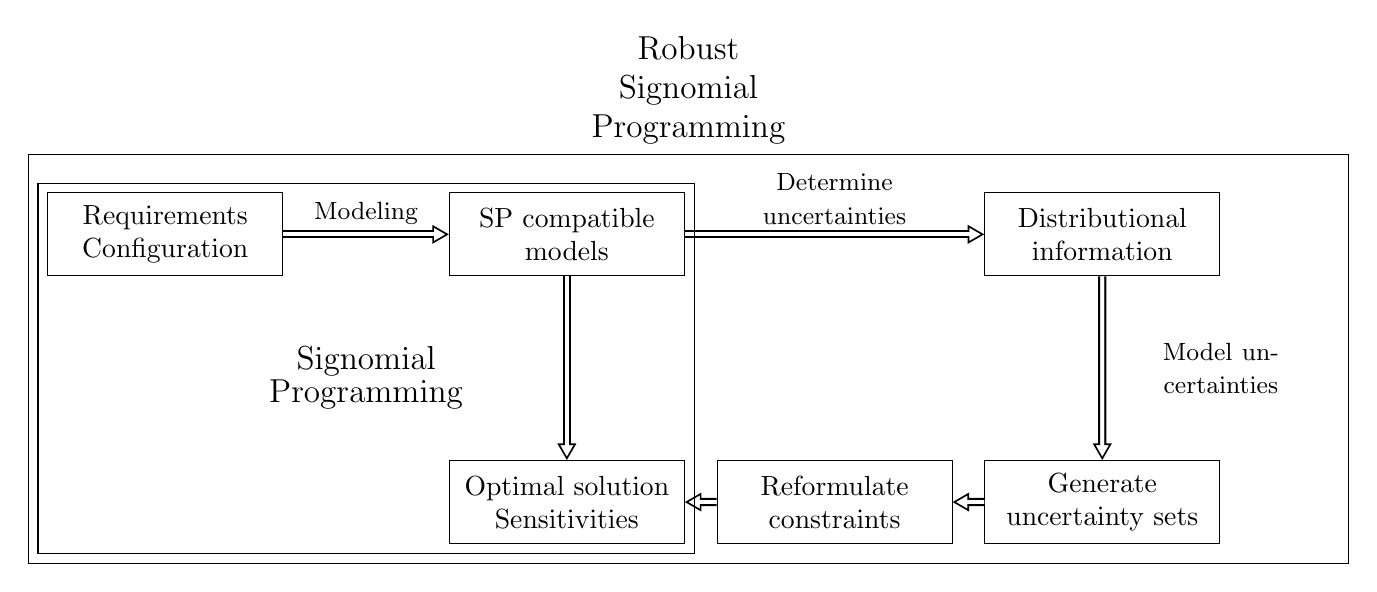
\begin{tikzpicture}[auto, align=center, text width=2.75cm, scale = 0.85]
        \begin{scope}[node distance=2cm]
        \node[block, name=reqs] at (0,0) (reqs) {Requirements \\ Configuration};
        \node[block, name=SPmodels] at (6,0) (SPmodels) {SP compatible \\ models};
        \node[block, name=optimum] at (6,-4) (optimum) {Optimal solution \\ Sensitivities};
        \node[block, name=distr] at (14,0) (distr) {Distributional \\ information};
        \node[block, name=sets] at (14,-4) (sets) {Generate \\ uncertainty sets};
        \node[block, name=reformulate] at (10,-4) (reformulate) {Reformulate constraints};
		\node[name=dummy] at (6, 0.5) (dummy) {};

		    \draw[vecArrow] (reqs) -- node[name=modeling] {\small Modeling} (SPmodels);
			\draw[vecArrow] (SPmodels)to (optimum);
			\draw[vecArrow] (SPmodels) -- node[name=detuncert] {\small Determine uncertainties} (distr);
			\draw[vecArrow] (distr) -- node[name=modeluncert] {\small Model uncertainties} (sets);
 			\draw[vecArrow] (sets) to (reformulate);
			\draw[vecArrow] (reformulate) to (optimum);

		\node[name=SP,label={[xshift=0.0cm, yshift=-3.0cm]\large Signomial Programming},fit=(reqs)(SPmodels)(optimum), draw] {};
		\node[name=RSP,label={[xshift=0.0cm, yshift=0.0cm]\large Robust \\ Signomial \\ Programming \\},
		fit=(SP)(reqs)(SPmodels)(optimum)(distr)(sets)(reformulate)(modeluncert)(detuncert)(modeling)(dummy), draw] {};
		\end{scope}
    \end{tikzpicture}
    \caption{A block diagram showing the difference between the design process using a \gls{sp} and a \gls{rsp}.}
        \label{fig:blockdiag}
\end{center}
\end{figure}

A \emph{\gls{sp} in exponential form} is as follows:
\begin{equation}
    \begin{split}
	\min & f_0\left(\mathbf{x}\right) \\
	\text{s.t.} & \textstyle{\sum}_{k=1}^{K_i}e^{\mathbf{a_{ik}}\mathbf{x} + b_{ik}} - \textstyle{\sum}_{k=1}^{G_i}e^{\mathbf{c_{ik}}\mathbf{x} + d_{ik}} \leq 0,~\forall i \in 1,...,m\\
\end{split}
\label{SP_exponential}
\end{equation}
where the constraints are represented as difference-of-posynomials in exponential form.
Let $\mathbf{a_{ik}}$ and $\mathbf{c_{ik}}$ be the $((i-1)\times m + k)^{th}$ rows of the exponents matrices
$\mathbf{A}$ and $\mathbf{C}$ respectively, and $b_{ik}$ and $d_{ik}$ be the $((i-1)\times m + k)^{th}$ elements
of the coefficients vectors $\mathbf{b}$ and $\mathbf{d}$ respectively.

The data ($\mathbf{A}$, $\mathbf{C}$, $\mathbf{b}$, $\mathbf{d}$) is assumed to be uncertain and
living in an uncertainty set $\mathcal{U}$, where $\mathcal{U}$ is parametrized
affinely by a perturbation vector $\mathbf{\zeta}$:
\begin{equation}
\mathcal{U} = \left\{\left[\mathbf{A};\mathbf{C};\mathbf{b};\mathbf{d}\right] = \left[\mathbf{A}^0;\mathbf{C}^0;\mathbf{b}^0\;\mathbf{d}^0 \right] +
\textstyle{\sum_{l=1}^{L}\zeta_l\left[\mathbf{A}^l;\mathbf{C}^l;\mathbf{b}^l; \mathbf{d}^l\right]}\right\}
\label{Data}
\end{equation}
where $\mathbf{A}^0$, $\mathbf{C}^0$, $\mathbf{b}^0$, and $\mathbf{d}^0$ are the nominal exponents and coefficients,
$\left\{\mathbf{A}^l\right\}_{l=1}^{L}$, $\left\{\mathbf{C}^l\right\}_{l=1}^{L}$, $\left\{\mathbf{b}^l\right\}_{l=1}^{L}$, and
$\left\{\mathbf{d}^l\right\}_{l=1}^{L}$ are the basic shifts of the exponents and coefficients,
and $\zeta_l$ is the $l^{th}$ component of $\mathbf{\zeta}$ belonging to a perturbation set $\mathcal{Z} \in \mathbb{R}^L$ such that
\begin{equation}
\mathcal{Z} = \left\{ \mathbf{\zeta} \in \mathbb{R}^L: \left\lVert \mathbf{\zeta} \right\rVert \leq \Gamma \right\}
\label{perturbation_set}
\end{equation}

As aforementioned, our goal is a formulation that is immune to
uncertainty in the data. Accordingly, the robust counterpart
of the uncertain \gls{sp} in \eqref{SP_exponential} is:
\begin{equation}
    \label{SP_counterparts_finite}
    \begin{split}
        \min & f_0\left(\mathbf{x}\right)\\
        \text{subject to} &\max_{\mathbf{\zeta} \in \mathcal{Z}} \left\{\textstyle{\sum}_{k=1}^{K_i}e^{\mathbf{a_{ik}}\left(\zeta\right)\mathbf{x} + b_{ik}\left(\zeta\right)} - \textstyle{\sum}_{k=1}^{G_i}e^{\mathbf{c_{ik}}\left(\zeta\right)\mathbf{x} + d_{ik}\left(\zeta\right)}\right\} \leq 1 \forall i \in 1,...,m\\
    \end{split}
\end{equation}

The optimization problem in \eqref{SP_counterparts_finite} is intractable using current solvers,
therefore,  a heuristic approach to solving \gls{rsp}s approximately
as a sequential \gls{rgp} will be presented in the following sections.
As our approach is based on robust geometric programming,
a brief review of the subject will follow based on \cite{Saab2018}.


\section{Robust Geometric Programming} \label{RGP}
In this section we will briefly review the approximation of an RGP as a tractable optimization problem as presented in \cite{saab2018} and \cite{hsiung_kim_boyd_2007}.

The robust counterparts of an uncertain geometric program is:

\begin{equation}
\begin{aligned}
& \min &&f_0\left(\vec{x}\right)\\
& \text{subject to} &&\max_{\vec{\zeta} \in \mathcal{Z}} \left\{\textstyle{\sum}_{k=1}^{K_i}e^{\vec{a_{ik}}\left(\zeta\right)\vec{x} + b_{ik}\left(\zeta\right)}\right\} &&\leq 1 &&\forall i \in 1,...,m\\
\end{aligned}
\label{GP_counterparts_finite}
\end{equation}

\subsection{Two Term Formulation}
 

\section{Approach to Solving Robust Signomial Programs}

This section presents a heuristic algorithm to solve a \gls{rsp}
based on our previous discussion on robust geometric programming.

\subsection{General \gls{rsp} Solver}
As aforementioned, a common heuristic algorithm to solve a \gls{sp} is
by sequentially solving local \gls{gp} approximations.
Similarly, our approach to solve a \gls{rsp} is based on solving
a sequence of local \gls{rgp} approximations. In Figure~\ref{fig:rspsolve},
we provide a step-by-step algorithm.
In this heuristic, a good initial guess will lead to faster
convergence and possibly a better solution.
The deterministic solution of the uncertain \gls{sp} is in general a good candidate $x_0$.

\begin{figure}
    \begin{center}
    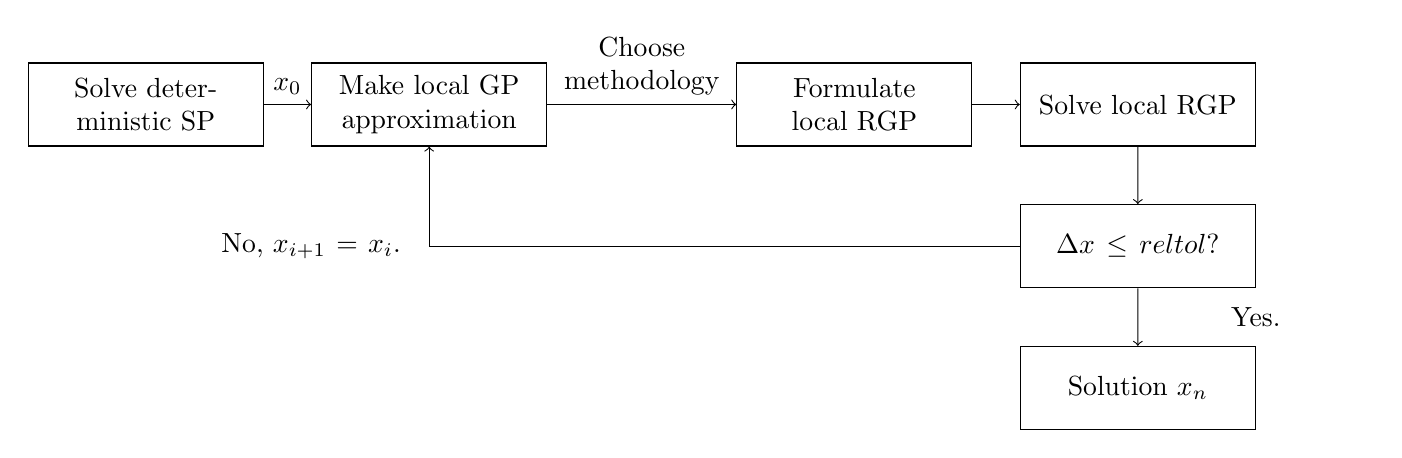
\begin{tikzpicture}[auto, align=center, text width=2.75cm, scale = 0.9]
        \begin{scope}[node distance=2cm]
        \node[block, name=detSP] at (0,0) (detSP) {Solve deterministic SP};
        \node[block, name=localGP] at (4,0) (localGP) {Make local GP approximation};
        \node[block, name=localRGP] at (10,0) (localRGP) {Formulate local RGP};
        \node[block, name=solveRGP] at (14,0) (solveRGP) {Solve local RGP};
        \node[block, name=xi] at (14,-2) (xi) {$\Delta x \leq reltol$?};
        \node[block, name=solution] at (14,-4) (solution) {Solution $x_{n}$};

        \draw[->] (detSP) -- node[name=x0] {$x_0$} (localGP);
        \draw[->] (localGP) -- node[name=choosemethod] {Choose methodology} (localRGP);
        \draw[->] (localRGP) -- (solveRGP);
        \draw[->] (solveRGP) -- (xi);
        \draw[->] (xi) -| node[name=no] {No, $x_{i+1} = x_i.$} (localGP);
        \draw[->] (xi) -- node[name=yes] {Yes.} (solution);
        \end{scope}
    \end{tikzpicture}
    \caption{A block diagram showing the steps of solving a \gls{rsp}.}
        \label{fig:rspsolve}
\end{center}
\end{figure}

For comparisons between methods ahead, we write the algorithm explicitly as follows:

\begin{enumerate}
    \item Choose an initial guess $x_0$.
    \item Repeat:
    \begin{enumerate}
        \item Find the local GP approximation of the \gls{sp} at $x_i$.
        \item Find the RGP formulation of the GP.
        \item Solve the RGP to obtain $x_{i+1}$.
        \item If $x_{i+1} \approx x_{i}$: break
    \end{enumerate}
\end{enumerate}

Any of the previously mentioned methodologies can be used to formulate the local RGP approximation. 
However, depending on the RGP formulation chosen to solve a \gls{rsp}, the formulation and solution
blocks in Figure \ref{fig:rspsolve} are adjusted.

\subsection{Best Pairs \gls{rsp} Solver}

If the Best Pairs methodology is exploited, then the above algorithm would change so that
each iteration would solve the local RGP approximation and choose the best permutation
for each large posynomial. The modified algorithm would become as follows:

\begin{enumerate}
    \item Choose an initial guess $x_0$.
    \item Repeat:
    \begin{enumerate}
        \item Find the local GP approximation of the SP at $x_i$.
        \item For each large posynomial constraint, select the new permutation $\phi$
                such that $\phi$ minimizes the robust large constraint evaluated at $x_i$.
        \item Solve the approximate tractable counterparts of the local \gls{gp} in
                \eqref{GP_counterparts_finite}, and let $\mathbf{x}_{i+1}$ be the solution.
        \item If $x_{i+1} \approx x_{i}$: break.
    \end{enumerate}
\end{enumerate}

\subsection{Linearized Perturbations \gls{rsp} Solver}

On the other hand, if the Linearized Perturbations formulation is to be used,
then we can avoid solving a \gls{sp} at each iteration by first
approximating the original \gls{sp} constraints locally, and in the same loop approximating
the robustified possibly signomial constraints locally, thus solving a
\gls{gp} at each iteration instead of a \gls{sp}. The algorithm would then become as follows:

\begin{enumerate}
    \item Choose an initial guess $x_0$.
    \item Repeat:
    \begin{enumerate}
        \item Find the local GP approximation of the SP at $x_i$.
        \item Robustify the constraints of the local GP approximation using the Linearized Perturbations methodology.
        \item Find the local GP approximation of the resulting local SP at $x_i$.
        \item Solve the local GP approximation above to obtain $x_{i+1}$.
        \item If $x_{i+1} \approx x_{i}$: break.
    \end{enumerate}
\end{enumerate}


\section{Models}

We implement the \gls{rsp} formulation above on an unmanned, gas-powered
aircraft design problem that is systematically developed in~\cite{Ozturk2018},
with the elliptical fuselage model borrowed from ~\cite{Burton2018}.
We optimize a wing, fuselage, and engine given a payload and range requirement.
The optimization model was developed using GPkit, a Python package that
provides abstractions for using \gls{gp}s in engineering design~\cite{gpkit}, and
captures fundamental trade-offs in aircraft design.
The nominal model has 175 variables and 153 constraints, a common level of
sparsity for~\gls{gp} and~\gls{sp} models.
A short qualitative overview of the model follows; for
more detailed information, please refer to~\cite{Burton2018} and~\cite{Ozturk2018}. The uncertainties
associated with the parameters will be described in Section~\ref{uncertainties_and_sets}.

\subsection{Flight Profile}

The flight profile model is borrowed from ~\cite{York2018}. Within the model, the
trajectory of the aircraft is optimized over four steady flight segments,
although we only model climb segments
and therefore the stored gravitational potential energy of the aircraft is not captured.

\subsection{Atmosphere}

The atmosphere model is taken from~\cite{Tao2018}, and considers changes in density and dynamic
viscosity with altitude, for a standard atmosphere.

\subsection{Aircraft}

The aircraft is modeled as a wing, fuselage and engine system. The aircraft is assumed
to be in steady flight, so that the thrust power is equal to the sum of the drag power and rate of change
of potential energy of the aircraft, and the lift is equal to the total weight, ignoring the vertical component of
thrust in climb. Its total weight is the sum of its components.
The aircraft has to be able to takeoff at specified minimum speed without stalling as well.
Aircraft component models are detailed below.

\subsubsection{Wing}

Lift is generated by the wing as a function of its geometry and free stream conditions.
The wing structure model is based on a beam model with a distributed lift load,
and a point mass in the center representing the fuselage.
Wing fuel volume is modeled as a fraction of the internal volume available in the wing.
The weight of the wing is the sum of skin and spar weights.
Its drag is the sum of induced and profile drags, the latter of which is
constrained by a 3-term softmax-affine posynomial fit~\cite{Hoburg2016} of drag polars
generated in XFOIL~\cite{XFOIL}.
The airfoil used was designed by Prof. Mark Drela of MIT and
is a variant of those implemented in~\cite{Burton2018}.

\subsubsection{Fuselage}

The fuselage contains the fuel and payload internally, and the engine externally.
It is assumed to be ellipsoidal in shape, and its drag is estimated using a form factor.
The fuselage is assumed not to contain any structural members, and so its weight consists only of skin weight.

\subsubsection{Engine}

The aircraft is powered by a naturally aspirated piston engine. It is subject to
power lapse at lower air densities at higher altitudes. Engine weight versus maximum sea level power,
and brake specific fuel consumption versus thrust and altitude
are modeled using the posynomial fits of engine performance data from ~\cite{Ozturk2017}.

\subsection{Source of non-log-convexity: fuel volume}
The fuel models have been detailed in the previous sections, but it is noteworthy that
the signomial constraint in the optimization appears in the aircraft total fuel volume constraint,
as shown in Equation~\ref{eq:fuel}:
\begin{equation}
\label{eq:fuel}
V_{\mathrm{f}} \leq V_{\mathrm{f_{wing}}} + V_{\mathrm{f_{fuse}}}
\end{equation}
The signomial constraints makes the problem non-log-convex, which means that the solution methods
detailed by Saab~\cite{Saab2018} need to be extended to accommodate this optimization problem.


\section{Uncertainties and Sets}
\label{uncertainties_and_sets}

As aforementioned in Section~\ref{sec:robustvsstochastic}, one of the advantages
of \gls{ro} over \gls{so} is the fact that it is more effective in absence of
data, since the problem has uncertainty set bounds on parameters as inputs instead
of complete probability distributions.
These uncertainties, given by three times the \gls{cv}\footnote{The \gls{cv}
is defined as follows: $\text{CV} = \frac{\sigma}{|\mu|}$, where $\sigma$ is the standard deviation and $\mu$ is the mean of the parameter.},
are listed in Table~\ref{tab:uncertainties}. Since for the rest of this work
all standard deviations ($\sigma$) are normalized by the means of the parameters, we will use $3\sigma$
to represent $3\text{CV}$.

\begin{table}
\begin{center}
\caption{\label{tab:uncertainties} Parameters and Uncertainties (increasing order)}
\begin{tabular}{c c c c c}
\hline
Parameters & Description & Value & \% Uncert. ($3\sigma$) \\
\hline
$S_{\rm{wetratio}}$ & wetted area ratio & 2.075 & 3\\
e & span efficiency & 0.92 & 3\\
$\mu$ & air viscosity (SL) & $1.78 \times 10^{-5}~\mathrm{kg/(ms)}$ & 4 \\
$\rho$ & air density (SL) & 1.23 $\mathrm{kg/m^3}$ & 5 \\
$C_{L_{\rm{max}}}$ & stall lift coefficient & 1.6 & 5\\
k & fuselage form factor & 1.17 & 10\\
$\tau$ & airfoil thickness ratio & 0.12 & 10\\
$N_{\rm{ult}}$ & ultimate load factor & 3.3 & 15\\
$V_{\rm{min}}$ & takeoff speed & 30 m/s & 20\\
$W_0$ & payload weight & 6250 N & 20\\
$W_{w_{\rm{coeff,strc}}}$ & wing structural weight coefficient & $2 \times 10^{-5}~1/\mathrm{m}$ & 20\\
$W_{w_{\rm{coeff,surf}}}$ & wing surface weight coefficient & 60 $\mathrm{N/m^2}$ & 20\\
\hline
\end{tabular}
\end{center}
\end{table}

In this case of a conceptual aircraft design with no prior data,
the parameter uncertainties reflect aerospace engineering intuition.
The wing weight coefficients $W_{w_{\rm{coeff,strc}}}$ and $W_{w_{\rm{coeff,surf}}}$,
and the ultimate load factor $N_{\rm{ult}}$ have
large $3\sigma$s because the build quality of aircraft components is
often difficult to quantify with a large degree of certainty.
The payload weight ($W_0$) has a large uncertainty for similar reasons,
since it is often developed concurrently with the aircraft.
Parameters that engineers take to be
physical constants (sea level air viscosity and density, $\mu$ and $\rho$) and those that can be determined or manufactured with a relatively
high degree of accuracy ($S_{\rm{wetratio}}$, $e$) have relatively low deviations.
Parameters that require testing to determine ($C_{L_{\rm{max}}}$, $V_{\rm{min}}$) have a level of uncertainty
that reflects the expected variance of empirical studies. However, note that
these quantities are ultimately picked by the designer using prior experience and data,
and the level of conservatism in the
design will be greatly affected by the chosen $3\sigma$s.


\section{Results}

We finally implemented our RSP heuristic algorithm on a simple aircraft design problem. 
In this problem, we conduct an aerostructural optimization of a wing and fuselage given a payload and a range requirement. 

% We implemented the RSP formulation ideas above on a simple aircraft design problem, with 12 uncertain variables,
% and a single signomial constraint. . A short overview of the model follows.

\subsection{Optimization Results}

The problem is optimized for different sizes of box and elliptical uncertainty sets
by varying the parameter $\Gamma$ as defined in Appendix \ref{LP_to_GP}.
The design variables are then fixed for each solution so that the design can be simulated for
1000 different realizations of the uncertain parameters in Table~\ref{tab:uncertainties}
to examine average design performance.\\

\begin{figure}[ht]
    \centering
    \captionsetup{justification=centering, font=small}
    \begin{subfigure}{0.49\textwidth}
        \centering
        \includegraphics[height=2.3in]{signomial_simple_flight/box_best_pairs.png}
        % \caption{Box Uncertainty Set Objective Value}
    \end{subfigure}%
    ~ 
    \begin{subfigure}{0.49\textwidth}
        \centering
        \includegraphics[height=2.3in]{signomial_simple_flight/ell_best_pairs.png}
        % \caption{Box Uncertainty Set Probability of Failure}
    \end{subfigure}
    \caption{Performance of the optimal robust signomial simple aircraft, using the Best Pairs formulation, as a function of $\Gamma$ for different uncertainty sets.}
    \label{fig:probOfFailure}
\end{figure}

We can see from Figure \ref{fig:probOfFailure} that probability of failure goes to zero as $\Gamma$ increases.
Obviously, it is worth using elliptical uncertainty sets for this aircraft design problem as the performance is significantly better than that of a box uncertainty set, despite the increase in complexity. 
Moreover, using margins would in the best case be as good as using a box uncertaintyset, and therefore will lead to an inferior performance.

Figure~\ref{compare_signomial} compares the different methodologies in terms of run times, number of constraints, and average performance. The Best Pairs and Linearized Perturbations achieves good performance, however the Best Pairs methodology needs the most number of constraints, while the Linearized perturbations requires the most setup and solve time. The Simple Conservative formulation is significantly faster than the other formulations and requires the least number of additional constraints.
\ \\
\ \\

\begin{figure}[ht]
    \centering
    \captionsetup{justification=centering, font=small}
    \begin{subfigure}{0.499\textwidth}
        \centering
        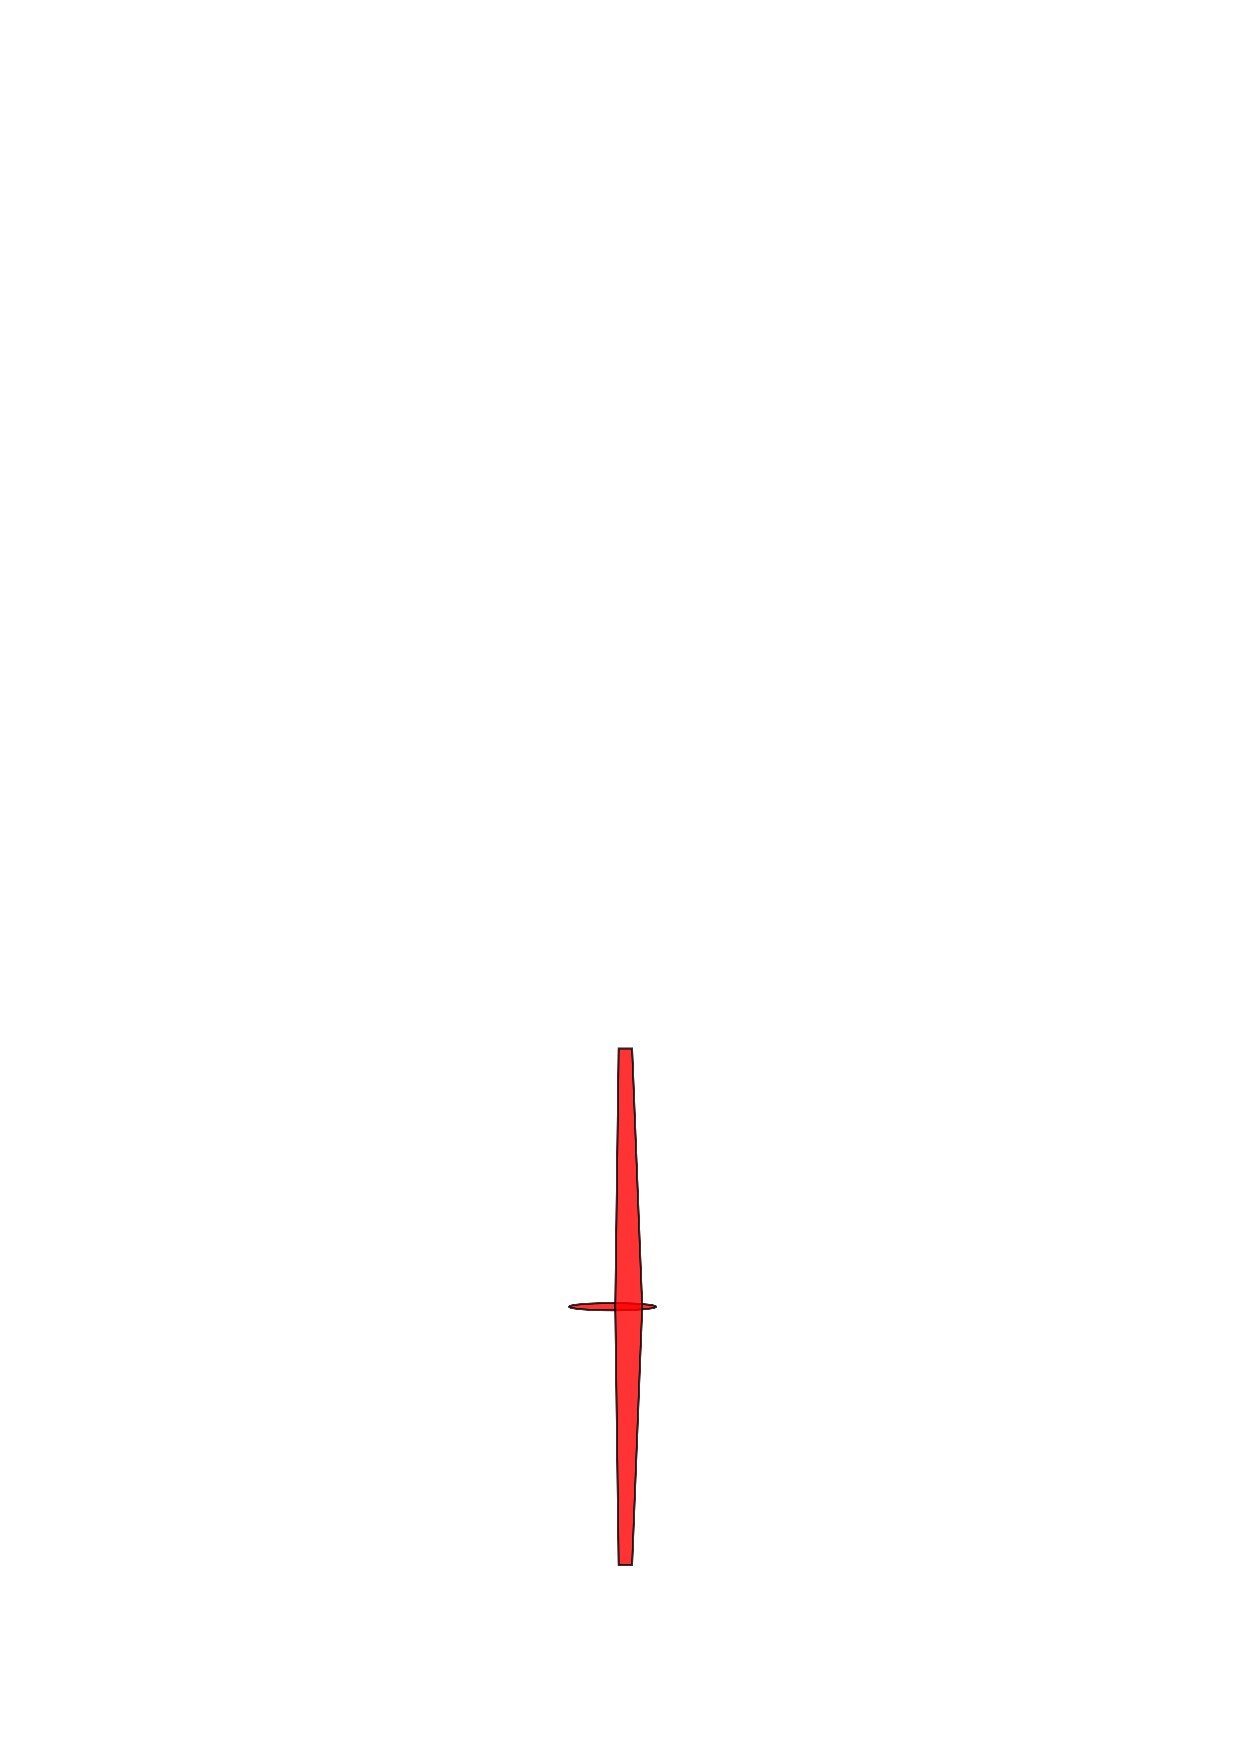
\includegraphics[height=2.3in]{signomial_simple_flight/box.png}
        % \caption{Box Uncertainty Set Objective Value}
    \end{subfigure}%
    ~ 
    \begin{subfigure}{0.49\textwidth}
        \centering
        \includegraphics[height=2.3in]{signomial_simple_flight/box_times.png}
        % \caption{Box Uncertainty Set Probability of Failure}
    \end{subfigure}
    ~
    \begin{subfigure}{0.499\textwidth}
        \centering
        \includegraphics[height=2.3in]{signomial_simple_flight/ell.png}
        % \caption{Elliptical Uncertainty Set Objective Value}
    \end{subfigure}%
    ~ 
    \begin{subfigure}{0.49\textwidth}
        \centering
        \includegraphics[height=2.3in]{signomial_simple_flight/ell_times.png}
        % \caption{Elliptical Uncertainty Set Probability of Failure}
    \end{subfigure}
    \caption{Robust signomial simple aircraft design results relative to the deterministic design problem.}
    \label{compare_signomial}
\end{figure}

\subsection{The Effect of Robustness}


%\textbf{TODO: update with 7-objective spider plots. First cite SP_tasopt, then show table and spider plots.
%Then show how robust results change the spider plots.}


One of the benefits of convex and difference-of-convex optimization methods is the ability to optimize for
different objectives~\cite{York2018}. For the aircraft model in question, we optimized for 7 different objectives, and show
the non-dimensionalized results in Table~\ref{tab:nondimresults}.

\begin{table}
    \resizebox{\textwidth}{!}{
    \csvautobooktabularcenter{figures/objective_table.csv}
    }
\caption{Non-dimensionalized variations in objective values with respect to the aircraft optimized
for different objectives. Objective values were normalized by the total fuel solution.}
    \label{tab:nondimresults}
\end{table}

To further demonstrate the capabilities of robust SPs in aircraft design,
we performed the optimization of the aircraft with no uncertainty and ellipsoidal uncertainty ($\Gamma = 1$)
for two more objective functions, and plotted the results on spider plots.
Spider plots are useful because they allow engineers to see the performance of different designs in a multi-objective
environment. Due to the large disparities in the potential values of design variables depending
on objective as shown in Table~\ref{tab:nondimresults}, we chose to demonstrate this using four objective functions
that would be expected to have a high degree of correlation and therefore yield similar aircraft designs. These were
 total (time and fuel) cost, total fuel, takeoff weight and mid-cruise lift-over-drag (L/D).

\begin{figure}
    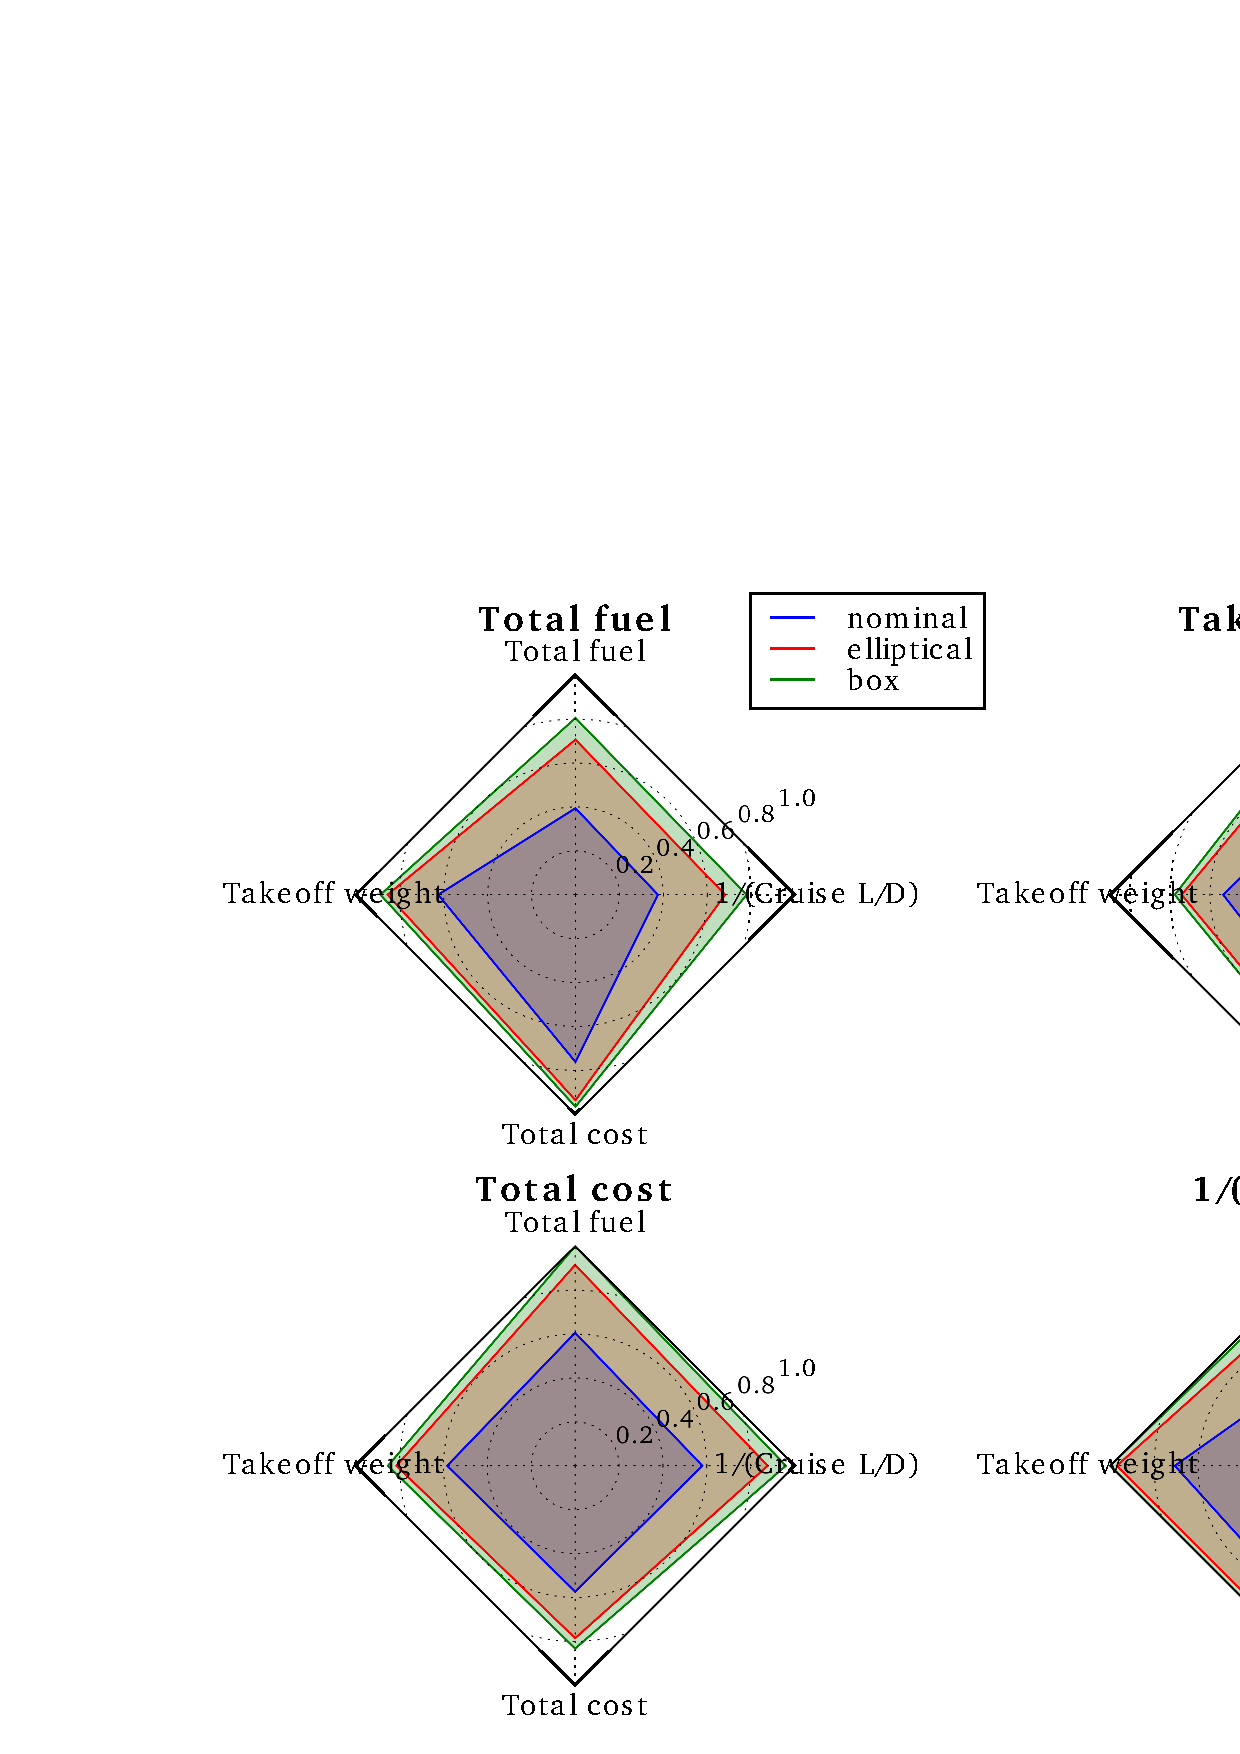
\includegraphics[width = 0.95\linewidth]{figures/4objradar.png}
    \caption{The spider plots of aircraft optimized for different objectives.
    The bolded titles are the design objectives for each plot, whereas the individual spiderwebs
    show the non-dimensionalized multiobjective performance of the aircraft designed under different
    uncertainty sets.}
    \label{fig:spider}
\end{figure}

In the spider plots in Figure~\ref{fig:spider}, it is possible to see the effect of robustness on
the different performance metrics of the different aircraft. One way to envision the multi-objective
performance of the aircraft is to consider the area contained within the web defined by the aircraft's
performance; the smaller the web area the beter.

For example, for the nominal case, which has no uncertainty, it is possible to see that
the aircraft designed for total fuel performs the best when all four objectives are considered.
However, this behavior changes when uncertainty is added. An aircraft optimized for total cost
(bottom left graph) with a box uncertainty set (in green) has better multiobjective performance
compared to an aircraft designed for total fuel with the same uncertainties.

This is an interesting result, because the presence of an uncertainty set is
shown to affect the efficacy of different objective functions to obtain solutions
with the best overall performance. If the three objective functions didn't
have high degree of coupling, that the internal areas of the solution triangles may differ
more significantly.

\subsection{Risk minimization problems}

All of the previous multi-objective analyses have assumed that we have an
understanding of exactly how much risk we are
willing to tolerate. This begs the question, could we have risk as the output of our
model? This would suggest the following formulation:

\begin{align*}
    \text{maximize} &~\Gamma \\
    \text{s.t.}     &~f_i(x,u) \leq 0, i = 1,\ldots,n \\
                    & \norm{u} \leq \Gamma \\
                    &~f_0(x) \leq (1+\delta)f_0^*,~\delta \geq 0 \tag{a}
    \label{eq:goalprogramming}
\end{align*}

where $f_0^*$ is the optimum of the nominal problem in Formulation~\ref{eq:normform}, $\delta$
is a fractional measure of the objective that we are willing to sacrifice for robustness, which
gives $(1+\delta)f_0^*$ as the upper bound on the objective value. Intuitively,
this is a form of goal programming,
where we specify the exact maximum worst-case value of an objective we can tolerate so that the program
risk is acceptable, but in the meanwhile maximize the total size of the uncertainty we can handle.

As a proof of the concept of this method, we can perform the same probability of failure
analysis as in Figure~\ref{fig:probOfFailure}, but have the objective bound be an input to the
optimization problem and the $\Gamma$ of the uncertainty set be maximized.

We can also expand this framework to perform multivariate goal programming,
by changing (a) in the formulation~\ref{eq:goalprogramming} to include all
objectives we are interested in.

\begin{align*}
    f_{0,j}(x) \leq (1+\delta_j) f^*_{0,j},~\delta_j \geq 0,~i = 1,\ldots, m
    \label{eq:multigoal}
\end{align*}

The benefit of goal programming is that it allows us to explore multidisciplinary tradeoffs without
having to enumerate the design space along each objective direction. Furthermore, in design it is not obvious whether
an objective should in fact be a constraint instead. For example, it's not clear that the design
of an aircraft is useful if it consumes

\subsubsection{Changes in flight envelope}


\section{Conclusion}

We have developed and applied a tractable \gls{rsp} formulation to a simple aircraft model,
and then discussed the benefits of having robust solutions. \gls{rsp} formulations extend
the tractable approximate RGP framework developed by Saab to non-log-convex problems,
and are a valuable contribution to the fields of robust optimization and difference-of-convex programming.\\

\gls{rsp}s have a wide variety of potential applications in engineering design.
Within the Hoburg Research Group in the Aerospace Computational Design Lab, during the past year we
have developed a commercial aircraft design \gls{sp} that has between 1700 and 8000 variables,
depending on the whether it is a single-point, or multi-point optimization.
We expect that using RO in this conceptual aircraft design will result in designs
that are more robust with respect to uncertainties in operational parameters,
such as payload mass and range, as well as uncertain constants.




\section*{Appendix}

\subsection{Robust Linear Programming: A Quick Review} \label{LP_to_GP}

As mentioned earlier, principles from robust linear programming are used
formulate an approximate robust geometric program.\\[12pt]
Consider the system of linear constraints
\begin{equation*}
    \mathbb{A}\vec{x} + \vec{b} \leq 0
\end{equation*}
where
\begin{equation*}
\begin{aligned}
\mathbb{A} &\text{ is $m \times n$}\\
\vec{x} &\text{ is $n \times 1$}\\
\vec{b} &\text{ is $m \times 1$}\\
\end{aligned}
\end{equation*}
where the uncertain data is contained in a set defined by equations \eqref{Data} and \eqref{perturbation_set}.

\subsubsection{Box Uncertainty Set}
If the perturbation set $\mathcal{Z}$ given in equation \eqref{perturbation_set} is a box
uncertainty set, i.e. $\|\vec{\zeta}\|_{\infty} \leq \Gamma$, then the robust formulation of the $i^{th}$ constraint is equivalent to
\begin{equation}
\Gamma \textstyle{\sum}_{l=1}^L |- {b}^l_{i} - \vec{a}^l_i\vec{x}| + \vec{a}^0_i\vec{x} + b^0_i \leq 0
\label{box_absolute}
\end{equation}
If only $b$ is uncertain, i.e. $A^l = 0~\forall l = 1,2,...,L$, then equation \eqref{box_absolute} becomes
\begin{equation}
\textstyle{\sum}_{l=1}^L \vec{a}^0_{i}\vec{x} + b^0_{i} + \Gamma \textstyle{\sum}_{l=1}^L |b^l_{i}| \leq 0
\label{box_coeff}
\end{equation}
which is a linear constraint.

On the other hand, if $A$ is uncertain, the equation \eqref{box_absolute} is equivalent to the following set of linear constraints
\begin{equation}
\begin{aligned}
\Gamma \textstyle{\sum}_{l=1}^L w^l_{i} + \vec{a}^0_{i}\vec{x} + b^0_{i} &\leq 0\\
- b^l_{i} - \vec{a}^l_{i}\vec{x} &\leq w^l_{i} &&\forall l \in 1,...,L\\
b^l_{i} + \vec{a}^l_{i}\vec{x} &\leq w^l_{i} &&\forall l \in 1,...,L\\
\end{aligned}
\label{box_linear}
\end{equation}

\subsubsection{Elliptical Uncertainty Set}
If the perturbation set $\mathcal{Z}$ is an elliptical, i.e. $\textstyle{\sum}_{l=1}^L\frac{\zeta_l^2}{\sigma_l^2} \leq \Gamma^2$,
then the robust formulation of the $i^{th}$ constraint is equivalent to
\begin{equation}
\Gamma \sqrt{\textstyle{\sum}_{l=1}^L \sigma_l^2(- b^l_{i} - \vec{a}^l_{i}\vec{x})^2} + \vec{a}^0_{i}\vec{x} + b^0_{i} \leq 0
\label{ell_absolute}
\end{equation}
which is a second order conic constraint.

If only $b$ is uncertain, i.e. $\mathbb{A}^l = 0 \quad \forall l = 1,2,...,L$, then equation \eqref{ell_absolute} becomes
\begin{equation}
\textstyle{\sum}_{l=1}^L \vec{a}^0_{i}\vec{x} + b^0_{i} + \Gamma \sqrt{\textstyle{\sum}_{l=1}^L \sigma_l^2(b^l_{i})^2} \leq 0
\label{ell_coeff}
\end{equation}
which is a linear constraint.

\subsubsection{Norm-1 Uncertainty Sets}

If the perturbation set represented by $\mathcal{Z}$ is a norm-1 uncertainty set, i.e. $\|\vec{\zeta}\|_1 \leq \Gamma$,
then the robust constraint is
\begin{equation}
\textstyle{\sum}_{l=1}^L \vec{a}^0_{i}\vec{x} + b^0_{i} + \Gamma \max_{l=1,..,L} |b^l_{i}| \leq 0
\label{rom_coeff}
\end{equation}
when $\mathbb{A}^l = 0$, and 
\begin{equation}
\begin{aligned}
\Gamma w_{i} + \vec{a}^0_{i}\vec{x} + b^0_{i} &\leq 0\\
- b^l_{i} - \vec{a}^l_{i}\vec{x} &\leq w_{i} &&\forall l \in 1,...,L\\
b^l_{i} + \vec{a}^l_{i}\vec{x} &\leq w_{i} &&\forall l \in 1,...,L\\
\end{aligned}
\label{rom_linear}
\end{equation}
if $\mathbb{A}^l \neq 0$. Note that for this type of uncertainty, the robust constraints are linear.


\section*{Acknowledgments}

A place to recognize others.

\bibliographystyle{aiaa}
\bibliography{main}

\end{document}

% - Release $Name:  $ -
